\begin{figure}[H]
	\centering
	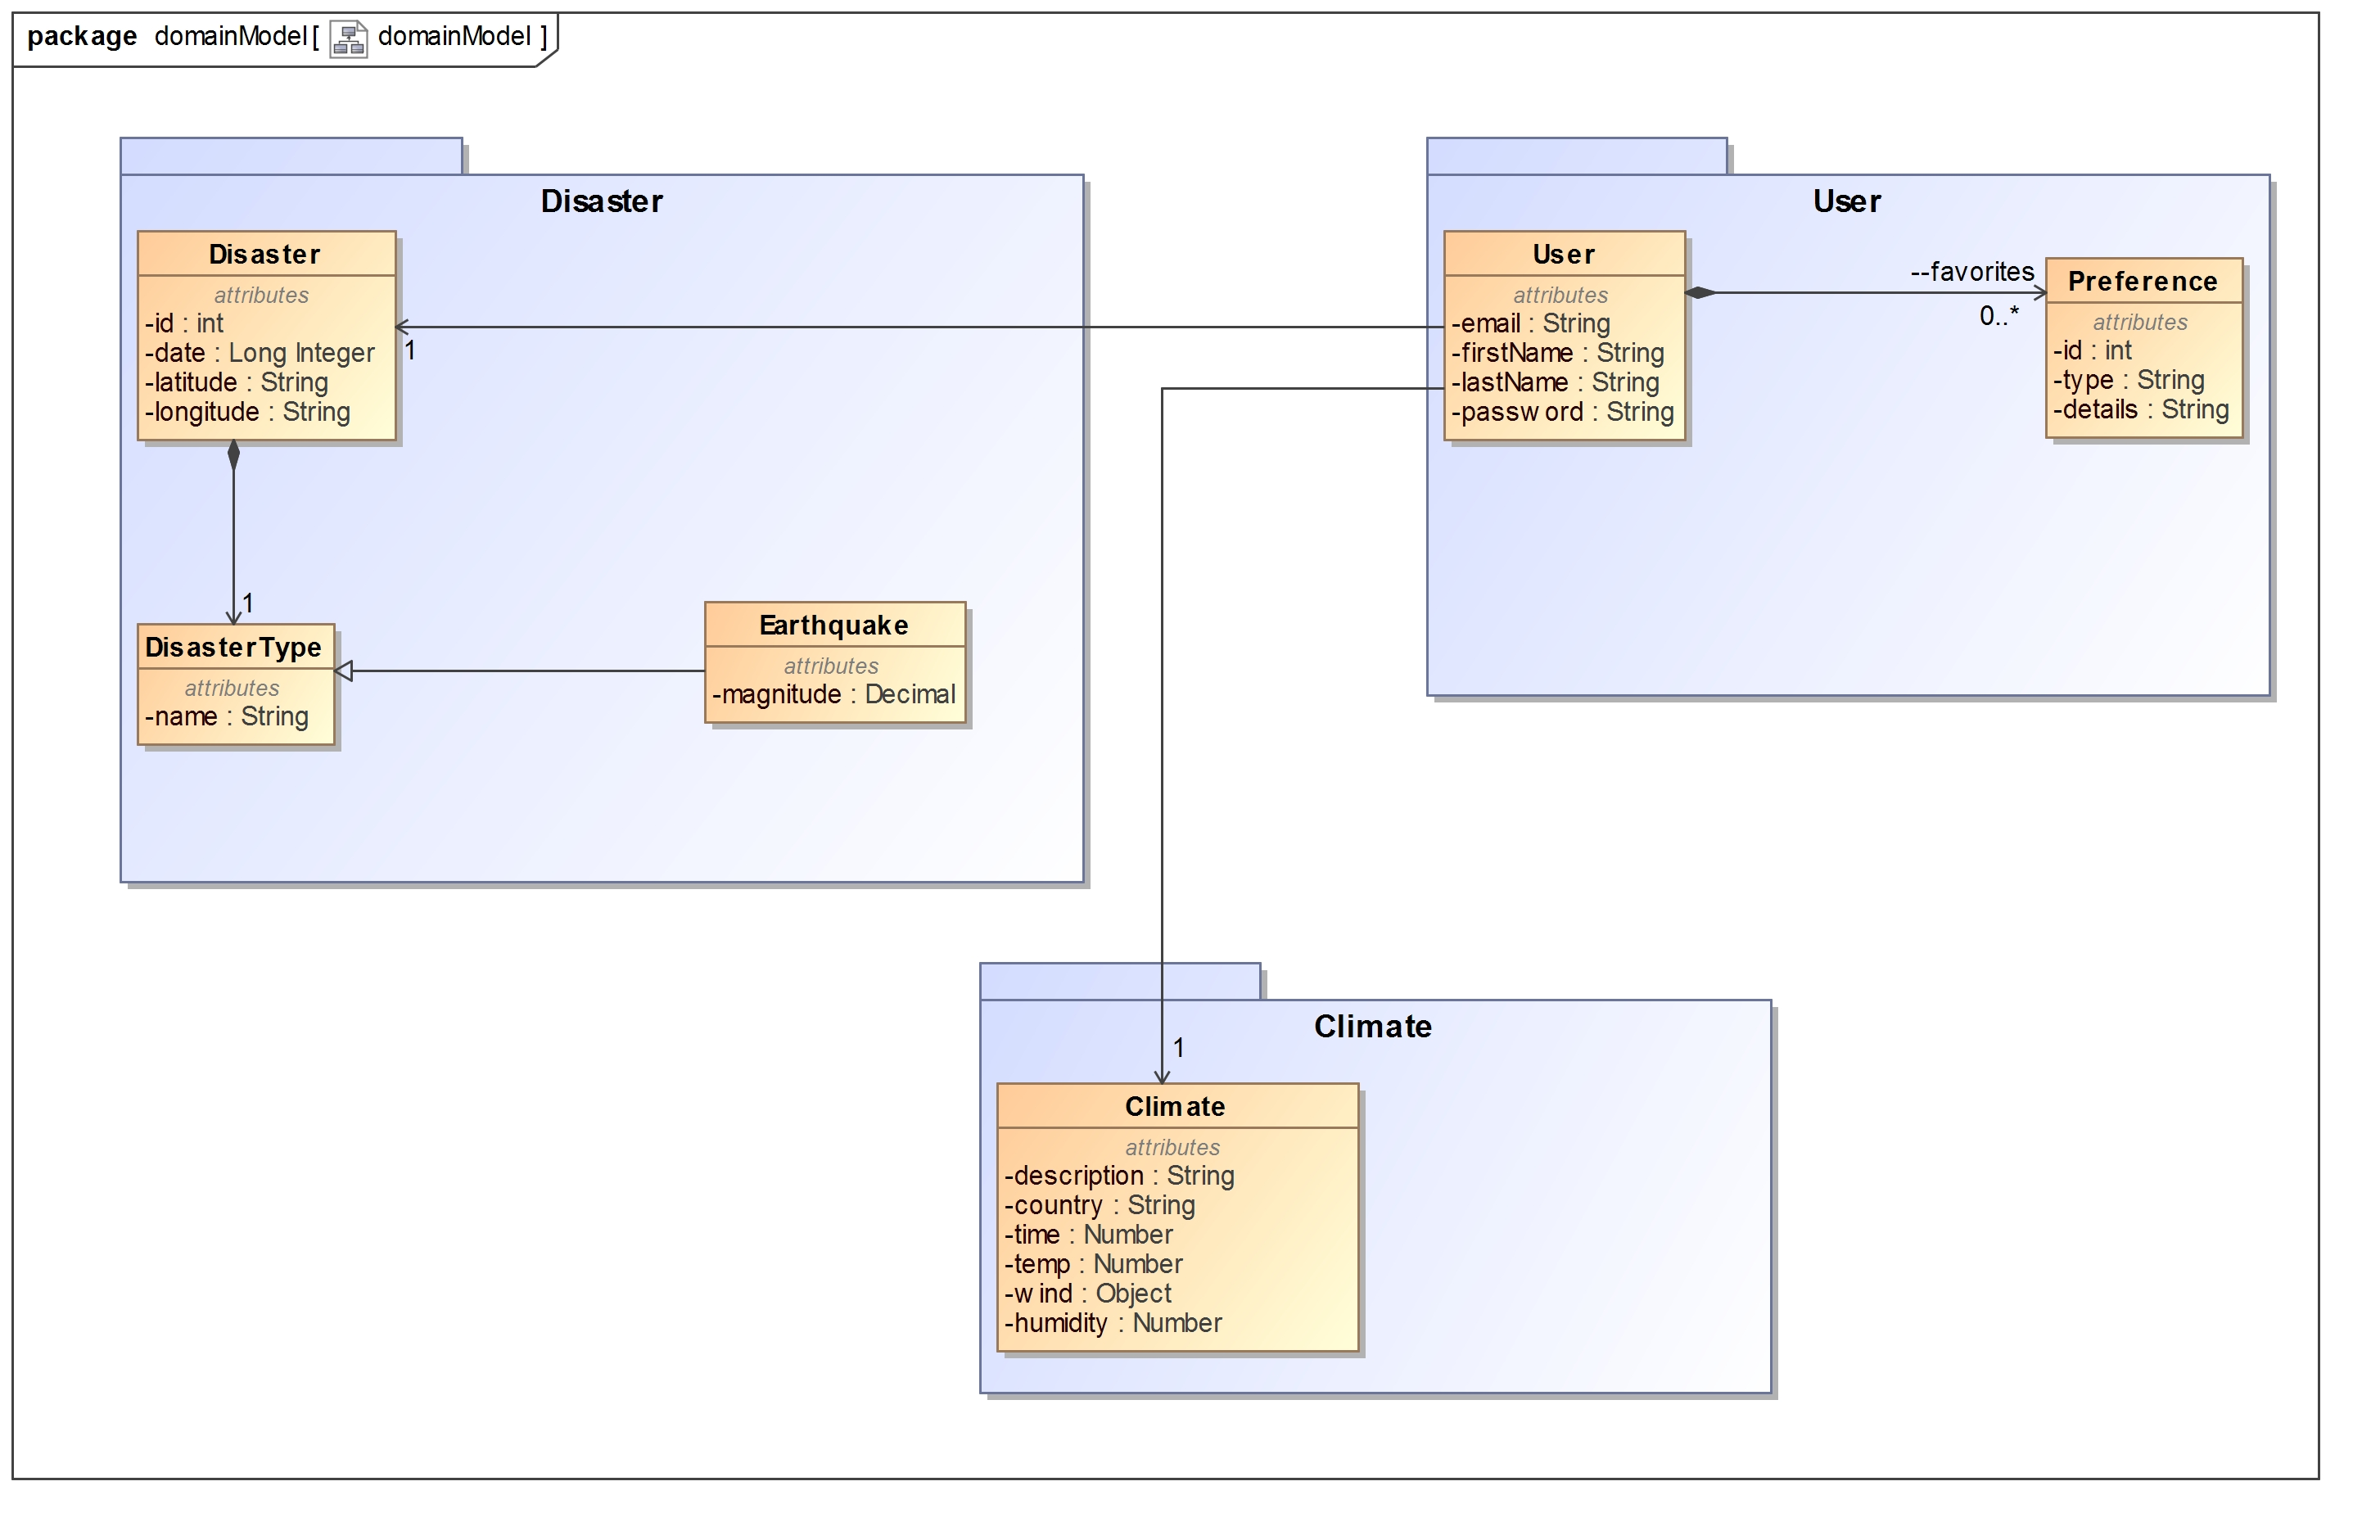
\includegraphics[scale=0.17]{../images/funcReq/domainModel.jpg}
	\caption{The domain model for the climate, disaster and user modules \label{overflow}}
\end{figure} Each user has a first name, last name, password and an email address. A user can also have 0 or more favourites that they can save by specifying the type of preference (disaster or weather) as well as other required details identifying the type of preference. A user, who is a client, is able to request services from the disaster and climate system components. A disaster which has an id, latitude, longitude, date and extra details also has a type. A disaster type could either be a fire, earthquake, flood or etc but at current the system has earthquake as the only type. Climate, on the other hand has a description, and values describing the country, time, temperature, wind and humitidty of a specific climate.